%%%%%%%%%%%%%%%%%%%%%%%%%%%%%%%%%%%%%%%%%%%%%%%%%%%%%
\chapter{Introduction} \label{chap:intro}
\graphicspath{{images/intro/}}

\ES{Should I frame it as an HRI problem? - alternative: remove first two sentences and update the end}

\gls{hri} explores the challenges of developing robots to interact in human environments and how human beings react to such robots. While not being present in every home yet, robot are quickly propagating through society, for instance as vacuum cleaner, pets, assistants or even friends \cite{belpaeme2012multimodal}. 
To interact in human environments robots require a way to make sense of their sensory inputs and act on the social world, they need to be sociable \citep{breazeal2004designing}. However, interacting socially with humans is a complex task: the social interaction happens on multiple levels and combines elements from multiple fields \citep{fong2003survey} and social norms used by humans are also transferred to robots \citep{bartneck2004design}. Providing robots with such a complex action policy is challenge, and will not be solved by programming by hand a static controller covering all the possible aspects and conditions. To interact meaningfully with humans, robots need to learn, constantly expanding and refining their action policy. We propose using the experts in humans interactions, the humans themselves to teach robot to interact socially. By providing control over the robot's actions to a human teacher, robots could learn efficient policies for social interactions from in-situ human supervision. Interactively learning from humans presents a change of paradigm compared to traditional machine learning, the human has an opportunity to guide the learning to make it more efficient \citep{feil2005defining,amershi2014power}. Furthermore, by initially framing this work in the context of \gls{hri} we added to the interaction a large set of constraints; consequently a method working in such a complex environment would have applications beyond \gls{hri} e.g. to \gls{ml} and \gls{ai}.

\ES{maybe the reopening is abrupt, might be worth going more in depth about what we have been doing}

%what it is and why it matters and why it is challenging
%
%Robots will inhabit human spaces and need to interact with them in decent ways
%
%Robot behaviour unlikely to be programmable and static
%
%This works explores how robots could interact with humans to learn from them to interact with other humans

%%%%%%%%%%%%%%%%%%%%%%%%%%%%%%%%%%%%%%%%%%%%%%%%%%%%%
\section{Scope}\label{sec:intro-scope}

As shown in \citep{goodrich2007human} only a subset of \gls{hri} is designed to be inherently social. Using Goodrich and Schultz's definition of \gls{hri}, an important part of the field does not treat robot as social agent, they might be asocial entities having a task to complete or simply tools used by humans. However, as demonstrated by \cite{fincannon2004evidence}, even when used as a teleoperated machine, robots still provoke social reaction and expectations from humans. \cite{fong2003survey} make, among others, the distinction between ``evocative robot'' and ``socially interactive robots''. Evocative robots rely on human tendency to anthropomorphise to succeed in their task while for ``socially interactive robots'' the social side of the interaction is key. However in \gls{hri}, the sociality of the interaction might not be intended but simply be a by-product of the interaction. As a consequence, in this work we will refer to ``social robots'' as robots interacting in humans environments and considered as ``social agents'' by the humans interacting with this robot. The intentions of the robot designer or the actual robot's sociality are of minor importance if the humans interacting with the robot projects social competencies or expectations on the robot. Regardless on the initial intentions, a robot interacting with humans needs to manage these expectations to ensure the safety and comfort of its human partners. In summary, as soon as a robot interacts with humans, the social side of the interaction needs to be taken into account, the robot needs to be able to interact socially. 

%As described by \cite{goodrich2007human}, \gls{hri} studies ``robotic system for use by or with humans'', consequently, it covers the full spectrum of interactions between humans and robots ranging from physical assistance and teleoperation to social companions. In \cite{fong2003survey}, authors refer to ``socially interactive robots'', as ``robot for which social interaction plays a key role''. As such, these socially interactive robots exclude robot interacting purely physically with humans, such as exoskeleton, physical rehabilitation or pure teleoperation as in robotic assisted surgery. However, even with robots not intended to behave socially, humans might create bonds and relationships \cite{fincannon2004evidence}. As such, this review extends the concept of ``socially interactive robots'' not only to robots designed to interact socially, but to robots eliciting social response from the hu

%if a robot is consider as a social agent, it needs to be able to interact socially

%social robots = robots perceived as social agents in human environments.

Enabling a robot to interact socially with humans is a complex task. The robot needs to make sense a large input space, from low level sensory feedback (e.g. joint angles or camera pixels) to high level concepts (e.g. hand-coded events or learned features). And based on the interpretation of these inputs and rules defining a behaviour, the robot needs to select an action or a plan to achieve an assigned goal. As this task covers most of the areas of robotics \cite{fong2003survey}, this section will precise the scope of the research conducted in this thesis.

\subsection{Frame}

The context of the research conducted here is finding a way for robots to interact efficiently with humans. It has been argued by many researchers  \citep{dautenhahn2004robots,billard2008robot} that robots need to adapt to their users and be able to learn from them. Social robots cannot apply a one-size-fits-all policy programmed in advance by engineers and suited to every possible interaction partners. Robots need the capability to learn an interactive behaviour, improving their skills as they interact in the world and personalising their policy to their users; and enabling such a learning is focus of this thesis.

Throughout this thesis we make the assumption that a human knows how the robot should interact. This `interactive knowledge' is not related to theoretical knowledge in \gls{ml}, robotics or other scientific fields but defines how the robot should behave. This that a person, generally not the engineers initially developing the robot, possesses some expertise which should be transferred to a robot. This expertise could take the form of the steps of a therapy a robot should deliver to the child (known by a therapist) or more simply a senior's preferences and desires concerning a robot companion's behaviour. As a consequence, robot users should be able to teach their robot, to transfer their knowledge to their robot without any technical expertise.

Although the ultimate goal of this research is to explore how robots could learn to interact socially and efficiently with humans; by making the assumption that the interactive knowledge should be provided by a human, the resulting question of this thesis is: \emph{How humans could teach robot to interact?}. As such, this research work aims to provide a convenient and efficient way for domain experts to inculcate robots with their interactive knowledge. In other words, this research explores the requirements on an interaction frameworks allowing humans to teach robot to interact socially in human environments and the impacts such a framework would have on the interaction.

%\subsection{Environment} 
\subsection{Type of Interactions}

As mentioned in the previous section, by focusing the research on using humans to teach robots, we add a second human-robot interaction to the application interaction: the interaction between the robot and the teacher. This results in two intertwined human-robot interactions: the application interaction, between the application target and the robot and the teaching interaction, between the teacher and the robot (cf. Figure \ref{fig:intro_setup}). The end goal of teaching interaction is to achieve high standards in the application interaction. This results in a general triadic interaction between a human target, a robot and a human teacher. 

\begin{figure}[ht]
	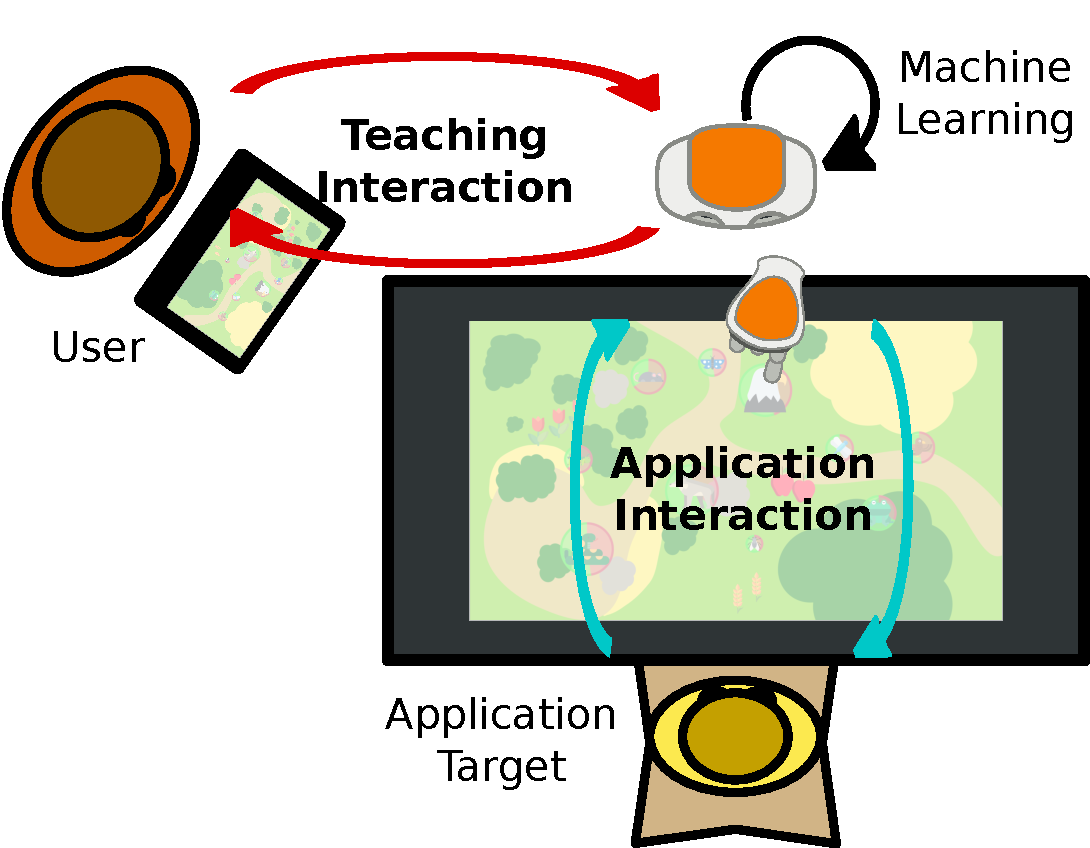
\includegraphics[width=.7\linewidth]{setup.pdf}
	\centering
	\caption{The typical interaction used in this research: a robot interacts with a target in an application interaction and learns from a domain expert through a teaching interaction.}
	\label{fig:intro_setup}
\end{figure}

While having been pursued by considering mostly \gls{hri} as an application interaction, the work presented in this thesis is applicable to teaching a robot, or more generally agents, many type of interactions, not only with humans. Indeed, interacting with a human is a high stake scenario, where misbehaving can be costly, where datapoints for learning can be tedious to acquire and with a high diversity between different partners. Other type of interaction could be less constrained, complex or with lower stakes. Consequently, by addressing a challenging task (teaching a robot to interact socially with humans), this approach is also be suited to a wide range of other tasks (such as manipulation, classification or navigation). In the more general case, the teacher or user of the robot has a task they would like the robot to complete. And through the teaching interaction, they can supervise the robot, demonstrating it what it should do and teaching it an efficient action policy in the application interaction with the target. 

%The application target could be another human (such as a child receiving teaching support from the robot) or just parts of the environment if the robot has to complete a manipulation of navigation task (such as picking up a book in the library).

%Mention more the social side of the interaction??

%Robots considered in this thesis evolve in human-centred environments and are expected to provide some support to the surrounding humans and achieve a specific goal assigned to them. Human interactions and by extend human environments are in essence social, they are governed by social norms, and on the adhesion to these norms depends the success of the interaction. 

%%%%%%%%%%%%%%%%%%%%%%%%%%%%%%%%%%%%%%%%%%%%%%%%%%%%%
\section{The Thesis}\label{sec:intro-thesis}
The main thesis this document seeks to put forward is as below.
\begin{quote}
	A robot can learn to interact meaningfully with humans in an efficient and safe way by receiving supervision from a human teacher in control of the robot's behaviour. 
	%This supervision will lead to an efficient, safe and low human-workload teaching and autonomous behaviour.	
\end{quote}
%One sentence to describe the take home/conclusion

Additional research questions have been explored during the progress of this
work and are introduced here.
%Maybe rephrase to remove constant "This research question..."
\begin{itemize}
	\item [RQ1] \textbf{What are the requirements of a robot controller to ensure a behaviour suited to \gls{hri}?} 
	
		By interacting with humans, robots enter the social world and have to conform to human expectations while ensuring they can reach their goal. This research question studies which constraints interacting in the human world put on the robot's controller. 
		
    \item [RQ2] \textbf{What interaction framework would allow a human to teach a robot while validating the requirements from RQ1?}
    
    	While RQ1 provides requirements for a robot controller, the task of designing a interaction framework allowing a human to teach remains. This research question address what principles of interaction could lead to an efficient teaching interaction whilst validating the requirements from RQ1. 
    	
    \item [RQ3] \textbf{Could a robot decrease its supervisor's workload by learning from their supervision?}
    
        Controlling a robot is a significant workload for the human supervisor. This question explores if including a learning component in the robot behaviour could alleviate the human workload by taking over some of the mental and physical requirements of the robot control and if this learning impacts the performance in the task.
%        \gls{woz} is an approach widely used in \gls{hri} \citep{riek2012wizard}, whereby a human teleoperates a robot to have it interact with other humans. However, this method applies a high workload on the operator and is not scalable. Using \gls{ml} to learn from this operator online might decrease the operator's workload without decreasing the quality of the robot behaviour.
    
    \item [RQ4] \textbf{How providing the teacher with control over the learner's actions impacts the teaching process?} 
    
    	Teaching robot has a unique property compared to teaching humans in the fact that the teacher could have total control over the learner's actions. This question explores if this control over the learner's action lead to faster, more efficient learning while being a lighter process for the teacher.
	%    In the context of \gls{iml}, a human can provide inputs to an agent to speed up the learning. Other \gls{iml} \citep{thomaz2008teachable,knox2009interactively} focus on feedback from the human with limited or no control over the agent's actions. However, increasing the control should speed up the learning and reduce the number of errors made by the robot.

	\item [RQ5] \textbf{How teaching a robot to interact socially impacts the two humans involved in the overall triadic interaction?}
%		How an interaction framework validating the requirements from RQ1 impact humans interacting with a robot when it is learning?}
	
		RQ2 explores how a teaching framework could in theory validate the requirements from RQ1. This questions studies if such a framework validates these requirements and its potential impact on the teaching process.
		%This research question evaluates if the framework proposed by exploring RQ2 would satisfy the requirements from RQ1 during the teaching process. 
		%Talk about impacts on both humans?
		
    \item [RQ6] \textbf{After receiving supervision from a human, could a robot behave autonomously in a social context?}
%    \item [RQ5] \textbf{How can a human teach a robot to interact with other humans?} %???

	 	After being taught, a robot can be deployed to interact autonomously in the real world. While RQ5 focused on the teaching phase, this questions analyses the robot's behaviour interacting autonomously and explores how efficient could the teaching be in providing the robot an autonomous behaviour validating principles from RQ1.
	 	%\gls{sparc} has been designed to allow non-experts in \gls{ml} to teach agents how to interact during the interaction. Human-robot interactions provide a perfect test for this approach: using a human to teach a robot how to behave in this complex and non-deterministic environment.
	 
\end{itemize}

%%%%%%%%%%%%%%%%%%%%%%%%%%%%%%%%%%%%%%%%%%%%%%%%%%%%%
\section{Approach and Experimentation}
\subsection{Thesis Overview} 
\ES{not sure if useful - cf structure}

%Big overlap with structure, but described the general flow of the thesis
To explore the thesis and the research questions addressed in this work, the first step was to review the field of application of social \gls{hri}. From this review, we addressed RQ1 by drawing three requirements for a robot to interact efficiently in human-environments. The robot constantly needs to have an appropriate action policy, be adaptive and require a low workload from humans. Then we reviewed the current controller for robots in \gls{hri} and identified the absence of a robot controller validating these requirements (cf. Chapter \ref{chap:background}).

In Chapter \ref{chap:sparc} we aimed to address this lack of method validating the requirements from Chapter \ref{chap:background}. To address RQ2, we proposed a new method, the \acrfull{sparc}, applicable to \gls{hri}. \gls{sparc} aims to provide control over the robot's action to a human and use this supervision to learn online a correct action policy. To achieve this goal, \gls{sparc} is based on a set of principles allowing this interaction to be efficient: the teacher can select actions for the robot, the robot can propose actions to the teacher, the teacher can pre-empt robot's propositions before an automatic execution and, finally, the robot learns from the teacher's selections and feedback to improve its action policy.

Once the method and the principles defining the interaction between the human teacher and the robot were set, we evaluated this approach in three studies with increasing ambition. Before testing \gls{sparc} in a real world interaction with humans (in Chapter \ref{chap:tutoring}), we needed to evaluate if the principles underlying \gls{sparc} could reduce the workload on the teacher (RQ3) and how the control over the robot's action impacts the teaching process (RQ4). The two first studies (Chapters \ref{chap:woz} and \ref{chap:control}) included humans only as teachers, but not as the target of the teaching. This allowed to gather initial information on \gls{sparc} in controlled and repeatable environments without having to tackle the challenges of interacting with humans in the real world.

%interaction between the teacher and the robot could lead to a learning of the robot side and a decrease of workload on the teacher side (RQ3) and if the control provided by \gls{sparc} improved the safety and the efficiency of the learning process (RQ4).

The first study, presented in Chapter \ref{chap:woz}, evaluated the interaction between the supervisor and the robot in a controlled and repeatable environment inspired by \gls{rat}. The study addressed RQ3 by exploring how the learning component of \gls{sparc} could reduce the teacher's workload by decreasing the number of actions required from the teacher.

Once \gls{sparc} demonstrated that it could allow a robot to learn and decreased the workload on the supervisor, we evaluated in Chapter \ref{chap:control} how the control provided to the teacher by \gls{sparc} could improve the learning process (RQ5). To explore the impact of such teacher's control, we designed a second study comparing \gls{sparc} to \gls{irl} an alternative approach used to teach robots, but providing the teacher with less control over the robot's action. Results showed that the control provided to the teacher help them to guide the robot to relevant parts of the environment, thus improving the teaching process.

Since the two first study demonstrated the efficiency of \gls{sparc} to teach a robot to interact in virtual environments, \gls{sparc} was ready to be evaluated in a real human-robot interaction: tutoring children in the wild. This last study applied \gls{sparc} to teach a robot a social and a technical policy to support child learning. This study had three main goals. First, demonstrating the applicability of \gls{sparc} in teaching robots to interact socially with humans, consequently addressing the thesis of this research. Secondly, exploring the impact during the teaching phase on the two humans involved in the triadic interaction (RQ5). And finally, evaluating if, after having been taught by a human using \gls{sparc}, the robot could interact successfully with other humans in an autonomous manner (RQ6).

%%%%%%%%%%%%%%%%%%%%%%%%%%%%%%%%%%%%%%%%%%%%%%%%%%%%%
%\section{Key Concepts and Terminology}\label{sec:intro-concepts}
%
%\subsection{Terminology}
%
%Not sure if worth including
%
%Throughout this thesis, the terms `wizard', `supervisor', `user', `expert' and `teacher' have been used interchangeably to represent the people in control of a robot's action and teaching that robot an action policy.
%
%agent and robot
%
%\begin{itemize}
%	\item \textbf{Appropriateness}:
%	\item \textbf{Adaptivity}
%	\item \textbf{Autonomy}
%	\item \textbf{Supervised Autonomy}
%	\item \textbf{Learning}
%	\item \textbf{Teacher, wizard, user, expert and supervisor}
%	\item \textbf{Robot, agent and learner}
%\end{itemize}

\subsection{Learning Algorithms}

\gls{ml} represents a subfield of \gls{ai} dedicated to exploring how statistical techniques can be used to provide artificial agents with learning. Two main categories of \gls{ml} are relevant this research: \gls{sl} and \gls{rl}.

\gls{sl} aims to learn a mapping between inputs and outputs to automatically reproduce a desired known behaviour. It uses a dataset of labelled example and optimises an algorithm to minimise the prediction error of labels \citep{russell2016artificial}. This aim, reproducing a desired behaviour, is especially connected with the work carried out in this research. By learning to reproduce the teacher's behaviour, the robot should reach an efficient behaviour in the target application. Typical example used in this study are \gls{ann} and nearest neighbours methods. \gls{ann} model loosely the way brains and neurons work by having a group of interconnected `neurons'. By changing the connections between the neurons, the network learns to reproduce the desired values on the output nodes according to the inputs provided. On the other hand, nearest neighbours methods are instance based methods, they compare the distance in the feature space between a point to classify and the different instances stored in a dataset and select the value of a majority of nearest neighbours in this space.

Unlike \gls{sl} which reproduces a known behaviours, \gls{rl} aims at providing an agent with the capacity to discover the world it interact in and learn from this interaction with the world \citep{sutton1998reinforcement}. The agent has access to a description of the state and actions it can do, and depending of the action selected, the state will change and the agent will receive a reward. The goal of the agent is to find an optimal policy maximising a notion of cumulated reward. \gls{rl} is also linked to the work presented in this thesis: by allowing robots to learn to interact in human environments, we would reach our goals of efficient human-robot interactions.

Due to the relevance of both fields to this thesis' research topics (enabling humans to teach robots to interact), algorithms from both categories have been used. The first study presented in Chapter \ref{chap:woz} used a feed forward neural network learning to reproduce a teacher policy. The second study in Chapter \ref{chap:control} used \gls{rl} to combine human guidance and environmental and human rewards to learn an efficient action policy. And the last study presented in Chapter \ref{chap:tutoring} used instance based algorithm adapted from Nearest Neighbours to enable online quick and efficient learning. More details about each algorithms and their related work can be found in the associated chapters.

\subsection{Data Analysis}

The data analysis in Chapters \ref{chap:control} and \ref{chap:tutoring} have been made using the Jasp software \cite{jasp2018} and the figures are generated using the seaborn package for Python and matplotlib \cite{waskom2017seaborn}. Jasp offers a Bayesian counterpart to classic statistical test, making them more robust and allowing to observe the presence or absence of effect. As such the Bayes factor $B$ is reported and represents how much of the variance on the metric is explained by a parameter (if $B < 1/3$ there is no impact, if $B > 3$ the impact is strong, and if $1/3<B<3$ the results are inconclusive; \citealt{jeffreys1998theory,dienes2011bayesian}). To represent data graphically, we used violin plots, they feature the kernel density estimation of the distribution.
%%%%%%%%%%%%%%%%%%%%%%%%%%%%%%%%%%%%%%%%%%%%%%%%%%%%%
%\section{Challenges}
%
%Complexity of interactions with humans: complex world, safety, workload and so on
%
%not sure if needed?

%%%%%%%%%%%%%%%%%%%%%%%%%%%%%%%%%%%%%%%%%%%%%%%%%%%%%
\section{Contributions}\label{sec:intro-contr}

\subsection{Scientific Contributions}
\begin{itemize}
	\item Design of \gls{sparc}, a new interaction framework for teaching agents in a safe way.
	\item Evaluation of \gls{sparc} in three studies.
	\item Demonstration of the importance of control over the robot's action when teaching a robot to interact.
	\item Design of a lightweight algorithm to quickly learn from demonstration in complex environments.
	\item Application of \gls{iml} to safely teach robots social autonomy from in situ human supervision. 
\end{itemize}

\subsection{Technical Contributions}
In addition to the scientific contributions, this research project lead to software development for multiple projects.
\begin{itemize}
	\item Development of three different studies to evaluate \gls{sparc} in three different scenarios (supervised robot-robot interaction, virtual robot and real word \gls{hri}).
	\item Partial development of a cognitive architecture and two tools for the \acrshort{dream} project (European FP7 project: 611391).
	\item Development of an autonomous robot controller to support cardiac rehabilitation in the Human-Robot Interaction Strategies for Rehabilitation based on Socially Assistive Robotics project (Royal Academy of Engineering: IAPP\textbackslash1516\textbackslash137).
	\item Development of a wizard interface for the Freeplay-Sandbox\footnote{\url{https://github.com/freeplay-sandbox}}. 
\end{itemize}
	
%%%%%%%%%%%%%%%%%%%%%%%%%%%%%%%%%%%%%%%%%%%%%%%%%%%%%
\section{Structure}\label{sec:intro-struct}
%From James, could probably be updated
The structure of this thesis is outlined below to provide an overview of the content and context for each chapter. A summary of key experimental findings are included at the start of each relevant chapter for ease of reference. 

\begin{itemize}
	%From James, could probably be updated
	\item This chapter provided an introduction to the general field of this research (robots learning to interact with and from humans), the research questions including the central \emph{thesis}, the scope and the contributions of the work presented in later chapters.  

	\item Chapter~\ref{chap:background} provides a description of the different fields of social \gls{hri} and draws three requirements for controllers of robots interacting with humans. In a second part, it analyses the current robot controllers used in \gls{hri} identifying that no current controller fits these requirements. Finally, it introduces \gls{iml} and proposes to apply it to \gls{hri} as a way to validate the requirements.
	
	\item Chapter~\ref{chap:sparc} proposes a new interaction framework, \gls{sparc}, as a way to apply \gls{iml} to \gls{hri} while validating the three requirements proposed in Chapter \ref{chap:background}. This chapter describes the principles behind \gls{sparc} and the expectations and limits this method could have.
	
	\item Chapter~\ref{chap:woz} presents results from a first study evaluating if \gls{sparc} would allow to reduce the workload on a supervisor compared to \gls{woz}. Results support the hypotheses, validating some of the motivations of \gls{sparc} (a learning robot would reduce the workload on a supervisor).
	
	\item Chapter~\ref{chap:control} presents results from a second study comparing \gls{sparc} to \gls{irl}, another interaction framework from \gls{iml}. The main difference between the two approaches is the amount of control the teacher has: with \gls{sparc}, the teacher can correct any action executed by the robot. Results from a 40 participants study support that this control improves the efficiency of the learning (improving the performance and time and inputs required to teach as well as decreasing the risks taken during the teaching phase).
	
	\item Chapter~\ref{chap:tutoring} presents the first study where \gls{sparc} has been applied to a real world \gls{hri}, child tutoring. Results demonstrate that, while not impacting the learning gain of the session, a supervised robot elicit richer child behaviour. By learning using \gls{sparc} an autonomous robot reach a similar policy than the supervised and achieved the same impact on the children. These results support \gls{sparc} as a teaching method allowing to transfer a social and technical action policy from human to a robot in a safe way and leading to efficient autonomous behaviour.
	
	\item Chapter~\ref{chap:discussion} presents a discussion from the main findings from the previous chapters and presents limitations and future directions of research for \gls{sparc}.
	
	\item Chapter~\ref{chap:conclusion} concludes the thesis and presents a summary of the main contributions.
	
\end{itemize}
